\documentclass[11pt, a4paper]{article}
\usepackage[utf8]{inputenc}
\usepackage[margin=1in]{geometry}
\usepackage{amsmath, amssymb, amsfonts}
\usepackage{graphicx}
\usepackage{booktabs}
\usepackage{xcolor}
\usepackage{hyperref}
\usepackage{tikz}
\usetikzlibrary{shapes, arrows, positioning}
\usepackage{pgfplots}
\pgfplotsset{compat=1.18}

% Title and Author
\title{Can Small Language Models Learn Matrix Inversion? \\
\large A Three-Level Diagnostic Study of Syntactic, Structural, and Functional Learning via Supervised Fine-Tuning}
\author{MatrixInvLLM Experimental Report}
\date{\today}

\begin{document}

\maketitle

% Abstract
\begin{abstract}
We investigate whether small language models (LLMs) can learn to compute matrix inverses through supervised fine-tuning on synthetic data---a controlled test of whether LLMs can internalize mathematical patterns that are computationally non-trivial for humans to reproduce from memory. Matrix inversion is an ideal probe: it has a verifiable ground truth ($AA^{-1} = I$), requires multi-step algebraic reasoning, and generates output that can look superficially plausible while remaining mathematically wrong.

Using LoRA (Low-Rank Adaptation, rank $r = 16$, $\alpha = 32$) to fine-tune Llama-3.2-3B on 800 supervised ($A$, $A^{-1}$) training examples covering $2 \times 2$ and $3 \times 3$ matrices, we evaluate both the untrained baseline and the fine-tuned model on 100 held-out examples using a multi-dimensional diagnostic suite that distinguishes three levels of success: (1) syntactic well-formedness, (2) coarse numeric resemblance to the true inverse, and (3) exact functional correctness via residual-based metrics.

Our main findings are:
\begin{itemize}
    \item \textbf{Baseline}: 100\% of outputs are syntactically parseable and correctly shaped, but 0\% satisfy the inverse constraint. All outputs are classified \texttt{NUMERICALLY\_WRONG}. Average residuals are $\|AX-I\|_F = 1.84$ and $\|XA-I\|_F = 1.85$. The model behaves essentially as a format imitator with no inverse-like numeric content (determinant ratio 0.045, sign agreement 0.503).
    \item \textbf{Fine-tuned}: Fine-tuning on 800 steps improves several coarse numeric diagnostics---determinant ratio rises from 0.045 to 0.639, sign agreement from 0.503 to 0.795, and relative Frobenius error to the gold inverse falls from 1.030 to 0.727---indicating partial internalization of inverse-like numeric structure. However, true inverse accuracy remains 0\% under all residual tolerances, and fine-tuning introduces severe generation instability: only 60\% of outputs are parseable, with 22\% entering repeated-block loops and 18\% producing malformed shapes.
\end{itemize}

The dominant conclusion is that LoRA fine-tuning learned \emph{partial inverse-like numeric structure} but could not bridge the gap to functional correctness, while simultaneously degrading generation reliability. This work provides a controlled diagnostic on the limits of supervised fine-tuning for precise arithmetic computation in small LLMs.
\end{abstract}


\newpage
\tableofcontents
\newpage

% Main Sections
\section{Introduction}

Large language models (LLMs) have demonstrated remarkable capabilities across language understanding and generation tasks. However, their ability to perform \emph{precise arithmetic reasoning}---especially on structured numeric problems with verifiable answers---remains poorly understood. A fundamental question is whether supervised fine-tuning can teach a model to internalize a mathematical \emph{function}, or whether it merely teaches the model to produce outputs that \emph{resemble} correct answers in format without satisfying the underlying constraints.

\subsection{Why Matrix Inversion?}

Matrix inversion is an ideal controlled benchmark for this question. Given a square matrix $A$, its inverse $A^{-1}$ is the unique matrix satisfying:
\[
A \cdot A^{-1} = I \qquad \text{and} \qquad A^{-1} \cdot A = I
\]
where $I$ is the identity matrix. Computing this by hand requires multi-step Gaussian elimination, careful row operations, and exact bookkeeping across $n^2$ entries---an operation that is cognitively demanding and error-prone for humans even at $3 \times 3$ scale. Yet the correctness of any candidate inverse $X$ can be verified instantly by checking the \emph{residual norms} $\|AX - I\|_F$ and $\|XA - I\|_F$.

This asymmetry---hard to produce, easy to verify---makes matrix inversion a valuable probe for studying whether LLMs can learn computationally demanding patterns from examples. If a model sees many ($A$, $A^{-1}$) pairs during training, can it distill implicit inverse-computation structure into its weights? Or does it learn only surface regularities, such as the output format or plausible value ranges, without satisfying the algebraic constraint?

\subsection{Research Question and Contribution}

We investigate: \emph{Can an LLM learn to compute matrix inverses through supervised fine-tuning on synthetic data, and what does the failure mode reveal about LLM arithmetic reasoning?}

To answer this, we design a rigorous experimental framework that:
\begin{enumerate}
    \item Generates 1{,}000 stable synthetic matrices ($2 \times 2$ and $3 \times 3$) with determinant and condition number filters to ensure well-posed inverse targets.
    \item Uses gold-standard residual validation ($\|AX - I\|_F < 10^{-8}$) rather than symbolic comparison.
    \item Employs deterministic text serialization for reproducible parsing and malformation detection.
    \item Fine-tunes Llama-3.2-3B using LoRA on 800 training examples for 800 optimization steps.
    \item Evaluates using a \emph{three-level diagnostic suite} distinguishing:
    \begin{itemize}
        \item \textbf{Syntactic well-formedness}: Is the output parseable into a valid matrix shape?
        \item \textbf{Inverse-like numeric structure}: Do coarse diagnostics (determinant ratio, sign agreement, relative Frobenius error) indicate the model has learned something about what inverses look like?
        \item \textbf{True inverse correctness}: Does the predicted matrix satisfy $\|AX - I\|_F < \varepsilon$ at any tolerance level?
    \end{itemize}
\end{enumerate}

\subsection{Key Findings}

Our results reveal a layered failure structure. The baseline (untrained) model produces syntactically valid output 100\% of the time but with no inverse-like numeric content. Fine-tuning substantially improves coarse diagnostics---the determinant ratio rises from 0.045 to 0.639, sign agreement from 0.503 to 0.795---suggesting that the model has internalized partial inverse-like structure. However, true inverse accuracy remains 0\% under all residual-based tolerances, and fine-tuning simultaneously introduces severe generation instability: only 60\% of fine-tuned outputs are parseable, with the remainder failing via repetition loops or malformed shapes.

The central finding is therefore not a simple ``format learned, function not learned'' story, but rather a \emph{graded partial learning} result: fine-tuning moved the model along the spectrum toward the target function without reaching it, and in doing so exposed a decoding reliability bottleneck that complicates interpretation.

\subsection{Paper Structure}

Section~\ref{sec:methodology} details our data generation, serialization, training setup, and the full evaluation metric suite. Section~\ref{sec:experiments} presents results across all three diagnostic levels. Section~\ref{sec:discussion} interprets the findings, discusses limitations, and outlines targeted future directions.


\section{Methodology}
\label{sec:methodology}

\subsection{The Core Scientific Question}

Our central hypothesis is that matrix inversion is a canonical example of a computation that is hard to produce algorithmically but easy to verify. A candidate inverse $X$ for input $A$ can be checked via the residual $\|AX - I\|_F$, making correctness unambiguous. The question we investigate is whether supervised fine-tuning can induce behavior consistent with approximate inverse computation in this setting---or whether the model learns only surface regularities such as output format and value ranges without satisfying the algebraic constraint.

We use a controlled synthetic setup to isolate this question from confounds such as ambiguous ground truth, label noise, or distribution mismatch.

\subsection{Matrix Generation and Stability Criteria}

We generate synthetic $n \times n$ matrices ($n \in \{2, 3\}$) by uniform random sampling from $[-1, 1]$, followed by stability filtering. To avoid ill-posed or numerically fragile inverse targets, we apply three criteria:

\begin{enumerate}
    \item \textbf{Determinant threshold}: $|\det(A)| > 0.05$. This threshold ensures full rank and avoids near-singular matrices whose inverses have extremely large entries; below this threshold, numerical precision in the target serialization would be insufficient to distinguish from degenerate cases.
    \item \textbf{Condition number bound}: $\kappa(A) < 50$. A condition number above this value implies that small perturbations in input encoding can produce large changes in the inverse, making the mapping harder to learn reliably. Both thresholds were chosen as conservative heuristic bounds based on standard numerical stability considerations.
    \item \textbf{Residual validation}: The computed gold inverse $X^*$ must satisfy $\|AX^* - I\|_F < 10^{-8}$, confirming that our ground truth is numerically sound.
\end{enumerate}

We sample up to 20{,}000 candidates per matrix size and retain 500 examples per size, for a total dataset of 1{,}000 examples.

\subsection{Data Serialization and Format}

Inputs and targets are serialized in a deterministic machine-readable text format. A representative example:

\begin{verbatim}
MatrixSize: 3
Matrix:
0.39195, -0.18209, -0.65341
-0.68713, -0.49951, 0.09845
0.42919, 0.32039, -0.44013
\end{verbatim}

\noindent The target output:
\begin{verbatim}
Inverse:
1.50708, -2.31690, -2.75565
-2.08222, 0.86379, 3.28444
-0.04613, -1.63052, -2.56829
\end{verbatim}

\noindent Design rationale: (1) Strict, exact headers (\texttt{MatrixSize:}, \texttt{Matrix:}, \texttt{Inverse:}) are required by the parser, enabling reliable detection of missing or malformed blocks; (2) Row-major, comma-separated ordering makes structural errors detectable; (3) Fixed 5-decimal precision balances floating-point accuracy with token length.

At inference time, the prompt is appended with the open header \verb|"\nInverse:\n"| so the model generates numeric rows directly, without needing to produce the header itself. Model outputs are post-processed by a truncation step that retains only the first valid \texttt{Inverse:} block, discarding any subsequent repetitions---this bounds the amount of looped content that reaches the parser. One known tradeoff is that strict header requirements may cause valid outputs to be classified as format failures if the model produces correct values with non-standard delimiters.

\subsection{Train/Val/Test Split}

We use a reproducible 80/10/10 split (seed = 123) across the full 1{,}000-example dataset:
\begin{itemize}
    \item \textbf{Train}: 800 examples
    \item \textbf{Validation}: 100 examples
    \item \textbf{Test}: 100 examples (48 of size $2 \times 2$, 52 of size $3 \times 3$)
\end{itemize}

The split is randomized across both matrix sizes jointly; it is not stratified separately by size. The test-set composition of 48 and 52 examples reflects the random split outcome, not a deliberate allocation. All reported results are on the held-out test set.

\subsection{Model and Training Setup}

\textbf{Base model}: Llama-3.2-3B \cite{llama32024}, a 3-billion-parameter decoder-only model.

\textbf{LoRA configuration}:
\begin{itemize}
    \item Rank: $r = 16$
    \item Alpha: $\alpha = 32$ (effective scaling factor $\alpha / r = 2$)
    \item Dropout: 0.05
\end{itemize}

\textbf{Optimization}:
\begin{itemize}
    \item Optimizer: AdamW ($\beta_1 = 0.9$, $\beta_2 = 0.95$)
    \item Learning rate: $5 \times 10^{-5}$ with 5\% linear warmup
    \item Weight decay: 0.01
    \item Training steps: 800 (batch size 16; 800 training examples are seen approximately once per step on average, giving roughly 1 epoch)
    \item Infrastructure: Tinker SDK with async pipelining
\end{itemize}

\textbf{Inference}: Greedy decoding (temperature = 0.0). Stop sequences include \verb|<|eot_id|>|, \verb|\nInverse:|, and \verb|\n\nInverse:|, which terminate generation when the model begins a second inverse block. The inference service imposed an effective ceiling of 4{,}096 tokens; as discussed in~\S\ref{sec:experiments}, all fine-tuned model outputs reached this ceiling. No hyperparameter search was performed; this is an intentionally minimal configuration.

\subsection{Evaluation Framework}

This paper is a diagnostic case study of one specific training configuration, not a comprehensive benchmark of LLM algorithmic capability. Results should be interpreted in that scope.

\subsubsection{Level 1 --- Syntactic Metrics}

\begin{itemize}
    \item \textbf{Parse success rate}: Percentage of outputs parseable into a valid matrix.
    \item \textbf{Shape correctness}: Among parseable outputs, percentage with correct dimensions ($n \times n$).
\end{itemize}

\subsubsection{Level 2 --- Coarse Numeric Diagnostics}

\textbf{Important caveat}: All Level 2 metrics are computed only on parseable (correct-shape) outputs. Baseline and fine-tuned Level 2 comparisons are therefore conditional on the respective parse-success subsets (100\% of examples for the baseline, 60\% for the fine-tuned model). Improvements in these metrics should be interpreted as improvements within the parseable subset, not as unconditional population-level improvements.

Metrics are averaged across all parseable examples pooled together (not stratified by matrix size unless noted).

\begin{itemize}
    \item \textbf{Relative Frobenius error}: $\|X - A^{-1}\|_F / \|A^{-1}\|_F$. Values near 0 indicate predictions close to the true inverse; a value near 1.0 indicates the error is roughly equal to the magnitude of the target itself.

    \item \textbf{Determinant ratio}: $\det(X) / \det(A^{-1})$. A perfect inverse satisfies $\det(A^{-1}) = 1/\det(A)$, so a ratio of 1.0 indicates correct determinant scale. A ratio near 0 indicates poor alignment with the target determinant scale.

    \item \textbf{Sign agreement}: Fraction of entries where $\mathrm{sign}(X_{ij}) = \mathrm{sign}(A^{-1}_{ij})$. A value near 0.5 is expected for random predictions over balanced distributions; higher values indicate improved alignment of predicted sign structure with the gold inverse.

    \item \textbf{Spectral error}: Largest singular value of $(X - A^{-1})$. Captures the magnitude of the dominant error direction, complementing the Frobenius norm.

    \item \textbf{Copy-detection distances}:
    \begin{itemize}
        \item $\|X - A\|_F$: Distance from the prediction to the input matrix.
        \item $\|X - A^T\|_F$: Distance from the prediction to the transpose of the input.
        \item $\|X - (-A)\|_F$: Distance from the prediction to the negation of the input.
    \end{itemize}
    These detect whether the model is producing a trivial transformation of its input rather than computing the inverse. Large values indicate the prediction is not a simple copy, though they must be read alongside other metrics to characterize what the prediction actually contains.
\end{itemize}

\subsubsection{Level 3 --- True Inverse Correctness}

\begin{itemize}
    \item \textbf{Left residual}: $\|AX - I\|_F$. Primary success criterion.
    \item \textbf{Right residual}: $\|XA - I\|_F$. Checks both-sided inverse consistency for square matrices; for an exact inverse, both residuals are zero.
    \item \textbf{Tolerance-based accuracy}:
    \begin{itemize}
        \item \textbf{Strict}: $\|AX - I\|_F < 10^{-2}$
        \item \textbf{Medium}: $\|AX - I\|_F < 5 \times 10^{-2}$
        \item \textbf{Loose}: $\|AX - I\|_F < 10^{-1}$
    \end{itemize}
    Passing even the loose tolerance would constitute evidence of approximate inverse behavior in this setup. All three failing simultaneously indicates the output is far from satisfying $AX \approx I$.
\end{itemize}

\subsubsection{Failure Mode Taxonomy}

We classify each output into one of six categories. Categories were defined a priori; some (EOS\_ONLY, PROMPT\_ECHO) were not observed in the reported run. When an output could in principle fit multiple categories, assignment follows the order below, with earlier categories taking precedence:

\begin{itemize}
    \item \texttt{EOS\_ONLY}: Output is empty after special-token removal.
    \item \texttt{PROMPT\_ECHO}: Output mirrors the input prompt verbatim.
    \item \texttt{REPEATED\_BLOCK\_LOOP}: Output enters repetition loops and exhausts the token budget without a complete matrix.
    \item \texttt{SHAPE\_FORMAT}: Output is partially parseable but has incorrect dimensions.
    \item \texttt{NUMERICALLY\_WRONG}: Correct shape, but residual $> 10^{-1}$ (loose tolerance failure).
    \item \texttt{SUCCESS}: Residual $< 10^{-2}$ (strict tolerance pass).
\end{itemize}

This taxonomy distinguishes \emph{decoding failures} from \emph{numeric failures}, making it possible to separate whether the bottleneck is generation reliability or mathematical computation.


\section{Experiments and Results}
\label{sec:experiments}

We evaluate both the untrained baseline and the LoRA fine-tuned Llama-3.2-3B on 100 held-out test examples (48 of size $2 \times 2$, 52 of size $3 \times 3$) across all three diagnostic levels described in~\S\ref{sec:methodology}.

\subsection{Baseline Behavior (Untrained Model)}

The untrained Llama-3.2-3B produces syntactically valid output on \textbf{100\%} of test examples---every output is parseable and correctly shaped. This is itself informative: the model has sufficient prior knowledge of the serialization format to emit matrix-like text without any fine-tuning.

However, syntactic success does not translate to mathematical success. Residuals are:
\[
\|AX - I\|_F = 1.835 \quad \text{and} \quad \|XA - I\|_F = 1.851 \quad \text{(avg.\ over 100 examples)}
\]
Both values are far above any acceptable tolerance, and numeric accuracy is 0\% under strict, medium, and loose thresholds alike. All 100 outputs are classified \texttt{NUMERICALLY\_WRONG}.

The extended diagnostics reveal further structure:
\begin{itemize}
    \item \textbf{Determinant ratio}: 0.045 --- the determinants of predicted matrices are roughly $1/22$\textsuperscript{nd} the scale of the true inverse's determinant. The model has no control over the determinant of its output.
    \item \textbf{Sign agreement}: 0.503 --- essentially at chance, meaning the model's predictions are no more sign-aligned with the true inverse than a random matrix.
    \item \textbf{Relative Frobenius error}: 1.030 --- predictions are as far from the true inverse, proportionally, as the inverse itself is from the origin. This confirms near-random numeric content.
    \item \textbf{Spectral error}: 5.015 --- the dominant direction of error is large, indicating no directional bias toward the true inverse.
    \item \textbf{Copy distances}: $\|X - A\|_F = 1.448$, $\|X - A^T\|_F = 1.585$, $\|X - (-A)\|_F = 2.119$. The relatively small $\|X - A\|_F$ compared to $\|X - (-A)\|_F$ suggests the baseline outputs may be loosely similar in magnitude to the input, though not as a simple copy.
\end{itemize}

\noindent\textbf{Summary}: The baseline model is a format-competent but numerically uninformed predictor. It produces the correct output \emph{structure} with no apparent relationship between input and output values.

\subsection{Fine-Tuned Model Behavior}

After LoRA fine-tuning (800 steps on 800 training examples), we observe two simultaneous effects: improvement in coarse numeric diagnostics, and degradation in generation reliability.

\subsubsection*{Generation Reliability}

Only \textbf{60\%} of fine-tuned outputs are parseable and correctly shaped (vs.\ 100\% baseline). The 40-percentage-point drop is distributed across two decoding pathologies:
\begin{itemize}
    \item \texttt{REPEATED\_BLOCK\_LOOP}: 22 examples (22\%) --- the model enters a repetition loop, exhausting the token budget without completing a valid matrix.
    \item \texttt{SHAPE\_FORMAT}: 18 examples (18\%) --- the model produces partial output with wrong dimensions.
\end{itemize}

Notably, the fine-tuned model hits the 4{,}096-token limit on \emph{every} example, compared to the baseline's typical 52--55 tokens per output. This suggests fine-tuning disrupted the model's length-control mechanism, causing over-generation rather than clean termination.

By matrix size: parse success is \textbf{70.8\%} for $2 \times 2$ and \textbf{50.0\%} for $3 \times 3$, indicating that larger matrices suffer more severe generation instability.

\subsubsection*{Numeric Diagnostics (among 60 parseable outputs)}

Despite the reliability drop, the fine-tuned model's parseable outputs exhibit meaningfully improved inverse-like structure:

\begin{itemize}
    \item \textbf{Determinant ratio}: 0.639 (vs.\ 0.045 baseline, $\Delta = +0.594$) --- the model now produces outputs with determinants much closer to the correct scale, a substantial improvement.
    \item \textbf{Sign agreement}: 0.795 (vs.\ 0.503 baseline, $\Delta = +0.292$) --- 79.5\% of predicted entries have the correct sign, well above chance. The model is learning which entries should be positive or negative.
    \item \textbf{Relative Frobenius error}: 0.727 (vs.\ 1.030 baseline, $\Delta = -0.303$) --- predictions are now roughly 27\% closer, proportionally, to the true inverse than the baseline.
    \item \textbf{Spectral error}: 3.829 (vs.\ 5.015 baseline, $\Delta = -1.186$) --- the dominant error direction has shrunk by 24\%.
    \item \textbf{Residuals}: $\|AX - I\|_F = 1.719$ (vs.\ 1.835 baseline), $\|XA - I\|_F = 1.480$ (vs.\ 1.851 baseline). The right residual improves more substantially.
    \item \textbf{Copy distances}: $\|X - A\|_F = 3.175$ (vs.\ 1.448 baseline, $\Delta = +1.727$) --- fine-tuned outputs are much farther from being a copy of the input. Similarly, $\|X - A^T\|_F$ and $\|X - (-A)\|_F$ both increase. This indicates the model has stopped producing input-like outputs and is generating genuinely different values, though those values still do not satisfy $AX = I$.
\end{itemize}

\subsubsection*{True Inverse Correctness}

Despite these improvements, inverse accuracy remains \textbf{0\%} under all tolerance levels (strict, medium, and loose). No parseable output satisfies $\|AX - I\|_F < 10^{-1}$.

\subsection{Comparative Summary and Failure Mode Analysis}

The complete comparison is shown in Table~\ref{tab:results}. Table~\ref{tab:failure_modes} breaks down the fine-tuned failure mode distribution.

The net picture from the deltas is:
\begin{itemize}
    \item Fine-tuning substantially reduced trivial copying behavior ($\|X - A\|_F$ rose from 1.45 to 3.18), consistent with the model learning that the inverse is \emph{different from} the input.
    \item Fine-tuning improved the model's representation of what an inverse \emph{looks like} at the level of sign, scale, and relative magnitude.
    \item But these improvements are insufficient to satisfy $AX \approx I$, meaning the learned structure is still too coarse or too inaccurate to yield valid inverses.
    \item And fine-tuning introduced a severe generation reliability penalty: a 40-point drop in parse rate, driven by looping and shape errors, that makes the fine-tuned model less deployable than the baseline at the output level.
\end{itemize}

\subsection{The Three-Level Gap}

The results illustrate a three-level gap between syntactic, structural, and functional success:

\begin{center}
\begin{tabular}{lcc}
\toprule
\textbf{Level} & \textbf{Baseline} & \textbf{Fine-Tuned} \\
\midrule
Syntactic (parse + shape) & 100.0\% & 60.0\% \\
Structural (sign agreement) & 50.3\% & 79.5\% \\
Functional (any tolerance pass) & 0.0\% & 0.0\% \\
\bottomrule
\end{tabular}
\end{center}

Fine-tuning closes the structural gap substantially but leaves the functional gap intact. The bottlenecks are insufficient numeric precision and, critically, a decoding instability that eliminates 40\% of outputs before they can even be evaluated.


\section{Discussion}
\label{sec:discussion}

The revised results complicate any simple interpretation. It is not accurate to say that the model learned only output formatting and no mathematical relationship between input and output. Several diagnostics improved in ways that suggest the fine-tuned model captured broad numerical regularities associated with the inverse, including scale, sign structure, and reduced similarity to the input matrix itself. At the same time, those improvements remain insufficient for task success. Matrix inversion is an unforgiving functional target: small entrywise deviations can yield large residual errors, and coarse resemblance does not guarantee algebraic correctness. The results point to a gap between approximate structural alignment and exact functional computation.

\subsection{Why the Functional Gap Persists}

Several plausible, non-exclusive explanations may account for the remaining gap. These explanations are not fully separable without further ablation experiments.

\begin{enumerate}
    \item \textbf{Insufficient training signal.} 800 examples and 800 steps may be insufficient for a 3-billion-parameter model to generalize a precise function. Matrix inversion requires entrywise precision across all 4 or 9 output values; a small error in any entry can propagate into a large residual.

    \item \textbf{Representation mismatch.} LLMs process token sequences without intrinsic numeric semantics. Each floating-point value is tokenized as a sequence of character-level tokens. The model must implicitly treat these as numeric quantities and compose them correctly---a form of reasoning not supported by standard language modeling objectives.

    \item \textbf{Absence of intermediate computation.} Matrix inversion by Gaussian elimination proceeds through structured intermediate steps. Supervised fine-tuning on final ($A$, $A^{-1}$) pairs provides no signal about these steps, requiring the model to learn a direct input-to-output mapping that may be beyond what a small model can approximate from examples alone.

    \item \textbf{Selection effects in Level 2 diagnostics.} The structural improvements reported in Section~\ref{sec:experiments} are measured over the 60\% of fine-tuned outputs that are parseable. These may not be representative of the full fine-tuned distribution: outputs that terminated cleanly enough to be parsed may systematically differ from those that looped or became malformed. The apparent improvements could be overstated if loop-prone examples would have shown weaker numeric alignment.
\end{enumerate}

\subsection{Decoding Instability}

Format instability remained a primary bottleneck in this evaluation. All 100 fine-tuned outputs reached the 4{,}096-token inference ceiling, compared to typical baseline outputs of 52--55 tokens. The model lost clean length-controlled termination on every example after fine-tuning.

One possible explanation is that LoRA updates pushed the model toward generating more structured numeric content, and this effort leads to over-generation when the model cannot converge to a well-formed output---producing repeated blocks or fragmented shapes. This explanation is speculative; the precise cause is not established by the current evaluation.

The practical consequence is significant. A model that shows improved numeric structure among parseable outputs, but generates parseable output on only 60\% of examples, provides no net improvement in aggregate correctness (0 successes in both cases). Format instability must be addressed before the numeric improvements are meaningful in any applied sense.

\subsection{Interpretation}

A useful summary is to distinguish three levels of competence. First, a model may produce text that is syntactically well formed. Second, it may produce numbers that reflect some broad properties of the target distribution. Third, it may produce outputs that satisfy the mathematical function being asked. In this study, LoRA fine-tuning appears to improve the second level without reliably achieving the third, while also degrading robustness at the first level for 40\% of test examples. This result is informative: it demonstrates that the gap between structural resemblance and functional correctness is real and not closed by this training approach.

The results are compatible with a capacity-limitation interpretation---a sufficiently large model or more targeted training might succeed---but they do not establish it. The failure could equally reflect a more fundamental limitation of text-based arithmetic supervision.


\section{Conclusion}

We investigated whether small language models can learn matrix inversion through supervised LoRA fine-tuning on synthetic data---a diagnostic case study, not a comprehensive algorithmic benchmark. Our three-level evaluation framework (syntactic, structural, functional) reveals a nuanced outcome.

\textbf{What succeeded}: Among parseable fine-tuned outputs, several coarse numeric diagnostics improved relative to the baseline. The determinant ratio rose from 0.045 to 0.639, sign agreement from 0.503 to 0.795, and relative Frobenius error to the gold inverse fell from 1.030 to 0.727. Parseable fine-tuned outputs were also substantially farther from trivial input copying ($\|X - A\|_F$: 1.45 $\to$ 3.18). These shifts indicate partial inverse-like structure in the fine-tuned model's parseable outputs, going beyond mere format imitation.

\textbf{What failed}: True inverse accuracy remained 0\% under all residual-based tolerances for both models. Fine-tuning also introduced severe generation instability: only 60\% of fine-tuned outputs were parseable (vs.\ 100\% baseline), with exactly half of $3 \times 3$ examples failing, distributed between repetition loops (22\%) and malformed shapes (18\%).

\textbf{Dominant bottlenecks}: The experiment reveals two compounding issues. First, \emph{insufficient numeric precision}: the model shows improved coarse alignment but cannot satisfy the algebraic constraint $AX \approx I$ at any tolerance. Second, \emph{generation instability}: every fine-tuned output reached the 4{,}096-token inference ceiling, indicating a breakdown in length-controlled termination that prevents reliable evaluation of numeric quality. Addressing reliability is a prerequisite before further numeric progress can be meaningfully assessed.

\textbf{Caveats}: All structural improvements are measured conditionally over the 60\% of fine-tuned outputs that are parseable; direct comparison with the fully parseable baseline is not strictly equivalent. Results represent a single training run without variance analysis.

\textbf{Outlook}: This result is a diagnostic, not a verdict. Future work should prioritize: (1) simplifying the output serialization format to reduce format-induced failures; (2) decoding stabilization to address looping; (3) small-scale overfitting experiments to separate model capacity limits from format and reliability bottlenecks; and (4) intermediate-step supervision that provides signal about the computation process, not only the final answer. Scaling experiments, model comparisons, and hyperparameter search are best pursued after reliability is established.


\begin{thebibliography}{9}

\bibitem{cobbe2021training}
Cobbe, K., Kosaraju, V., Bavarian, M., Chen, M., Jun, H., Kaiser, L., Plappert, M., Tworek, J., Hilton, J., Nakano, R., Hesse, C., \& Schulman, J. (2021).
\textit{Training verifiers to solve math word problems}.
arXiv preprint arXiv:2110.14168.

\bibitem{lora2021}
Hu, E. Q., Shen, Y., Wallis, P., Allen-Zhu, Z., Li, Y., Wang, S., Wang, L., \& Chen, W. (2021).
\textit{LoRA: Low-rank adaptation of large language models}.
arXiv preprint arXiv:2106.09685.

\bibitem{llama32024}
Dubey, A., Jauhri, A., Pandey, A., Kadian, A., Al-Dahle, A., Letman, A., \& others (2024).
\textit{The Llama 3 herd of models}.
arXiv preprint arXiv:2407.21783.

\end{thebibliography}

% Appendices: Tables and Figures
\newpage
\appendix

\section{Tables}

\begin{table}[h!]
\centering
\caption{Stability Criteria and Dataset Generation Statistics}
\label{tab:stability}
\begin{tabular}{lc}
\toprule
\textbf{Parameter} & \textbf{Value} \\
\midrule
Matrix sizes & $2 \times 2$ and $3 \times 3$ \\
Samples per size (target) & 500 \\
Total dataset size & 1{,}000 examples \\
Train / Val / Test split & 800 / 100 / 100 \\
Test set composition & 48 of size $2 \times 2$; 52 of size $3 \times 3$ \\
Random distribution & Uniform $[-1, 1]$ \\
Determinant threshold & $|\det(A)| > 0.05$ \\
Condition number bound & $\kappa(A) < 50$ \\
Residual tolerance (gold) & $\|AX - I\|_F < 10^{-8}$ \\
Max generation attempts & 20{,}000 per size \\
Decimal precision (serialization) & 5 \\
Split seed & 123 \\
\bottomrule
\end{tabular}
\end{table}


\vspace{1cm}

\begin{table}[h!]
\centering
\caption{Training Configuration and Hyperparameters}
\label{tab:training_config}
\begin{tabular}{lc}
\toprule
\textbf{Component} & \textbf{Configuration} \\
\midrule
Base model & Llama-3.2-3B \\
Adapter method & LoRA (Low-Rank Adaptation) \\
LoRA rank ($r$) & 16 \\
LoRA alpha ($\alpha$) & 32 \\
Effective scaling ($\alpha / r$) & 2.0 \\
Dropout & 0.05 \\
Optimizer & AdamW ($\beta_1 = 0.9$, $\beta_2 = 0.95$) \\
Learning rate & $5 \times 10^{-5}$ \\
Weight decay & 0.01 \\
Warmup ratio & 5\% \\
Training steps & 800 \\
Batch size & 16 \\
Training examples & 800 (all from train split) \\
Max sequence length & 2{,}048 tokens \\
Inference decoding & Greedy (temperature = 0.0) \\
Effective token ceiling (observed) & 4{,}096 tokens \\
Training infrastructure & Tinker SDK (async pipelining) \\
\bottomrule
\end{tabular}
\end{table}


\vspace{1cm}

\begin{table}[h!]
\centering
\caption{Full Diagnostic Comparison: Baseline vs.\ Fine-Tuned on Test Set ($n = 100$ examples; 48 of size $2 \times 2$, 52 of size $3 \times 3$). Extended metrics are computed over parseable outputs only (100 baseline, 60 fine-tuned). $\uparrow$ = higher is better; $\downarrow$ = lower is better.}
\label{tab:results}
\begin{tabular}{lrrr}
\toprule
\textbf{Metric} & \textbf{Baseline} & \textbf{Fine-Tuned} & \textbf{Delta} \\
\midrule
\multicolumn{4}{c}{\textit{Generation Reliability}} \\
Parse / shape rate & 100.00\% & 60.00\% & $-40.00$ pp \\
\midrule
\multicolumn{4}{c}{\textit{True Inverse Correctness (Level 3)}} \\
Accuracy --- strict ($\|AX-I\|_F < 10^{-2}$) & 0.0\% & 0.0\% & $+0.0$ pp \\
Accuracy --- medium ($< 5 \times 10^{-2}$) & 0.0\% & 0.0\% & $+0.0$ pp \\
Accuracy --- loose ($< 10^{-1}$) & 0.0\% & 0.0\% & $+0.0$ pp \\
Avg $\|AX - I\|_F$ $\downarrow$ & 1.8354 & 1.7191 & $-0.1163$ \\
Avg $\|XA - I\|_F$ $\downarrow$ & 1.8513 & 1.4800 & $-0.3713$ \\
\midrule
\multicolumn{4}{c}{\textit{Coarse Numeric Structure (Level 2, parseable only)}} \\
Avg relative $\|X - A^{-1}\|_F$ $\downarrow$ & 1.0301 & 0.7273 & $-0.3028$ \\
Avg determinant ratio $\uparrow$ & 0.0451 & 0.6390 & $+0.5939$ \\
Avg sign agreement $\uparrow$ & 0.5033 & 0.7949 & $+0.2916$ \\
Avg spectral error $\downarrow$ & 5.0149 & 3.8292 & $-1.1857$ \\
\midrule
\multicolumn{4}{c}{\textit{Copy-Detection Distances (parseable only)}} \\
Avg $\|X - A\|_F$ (input copy?) & 1.4476 & 3.1753 & $+1.7277$ \\
Avg $\|X - A^T\|_F$ (transpose copy?) & 1.5852 & 2.7599 & $+1.1747$ \\
Avg $\|X - (-A)\|_F$ (negation copy?) & 2.1186 & 3.9595 & $+1.8410$ \\
\bottomrule
\end{tabular}
\end{table}

\vspace{1.5cm}

\begin{table}[h!]
\centering
\caption{Fine-Tuned Model Failure Mode Breakdown ($n = 100$ test examples). The baseline has no looping or shape failures; all 100 baseline outputs are \texttt{NUMERICALLY\_WRONG}.}
\label{tab:failure_modes}
\begin{tabular}{lrr}
\toprule
\textbf{Failure Mode} & \textbf{Count} & \textbf{Percent} \\
\midrule
\texttt{NUMERICALLY\_WRONG} & 60 & 60.0\% \\
\texttt{REPEATED\_BLOCK\_LOOP} & 22 & 22.0\% \\
\texttt{SHAPE\_FORMAT} & 18 & 18.0\% \\
\texttt{SUCCESS} & 0 & 0.0\% \\
\midrule
Total & 100 & 100.0\% \\
\bottomrule
\end{tabular}
\end{table}


\newpage
\section{Figures}

\begin{figure}[h!]
\centering
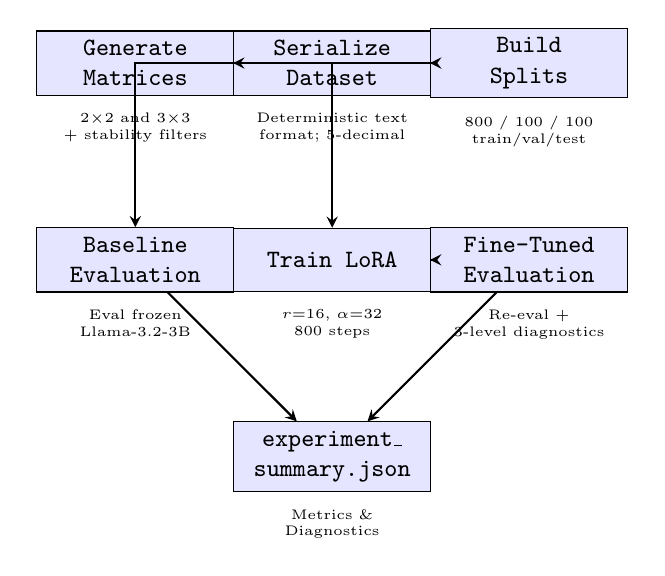
\begin{tikzpicture}[
    box/.style={rectangle, draw, fill=blue!10, minimum width=2.5cm, minimum height=0.8cm, font=\small\ttfamily, align=center},
    arrow/.style={->, >=stealth, thick},
    label/.style={font=\tiny, text width=2.5cm, align=center}
]

% Phase boxes
\node[box] (phase1) at (0,5) {Generate\\Matrices};
\node[label, below=0.1cm of phase1] {$2{\times}2$ and $3{\times}3$\\+ stability filters};

\node[box] (phase2) at (2.5,5) {Serialize\\Dataset};
\node[label, below=0.1cm of phase2] {Deterministic text\\format; 5-decimal};

\node[box] (phase3) at (5,5) {Build\\Splits};
\node[label, below=0.1cm of phase3] {800 / 100 / 100\\train/val/test};

\node[box] (phase4) at (0,2.5) {Baseline\\Evaluation};
\node[label, below=0.1cm of phase4] {Eval frozen\\Llama-3.2-3B};

\node[box] (phase5) at (2.5,2.5) {Train LoRA};
\node[label, below=0.1cm of phase5] {$r{=}16$, $\alpha{=}32$\\800 steps};

\node[box] (phase6) at (5,2.5) {Fine-Tuned\\Evaluation};
\node[label, below=0.1cm of phase6] {Re-eval +\\3-level diagnostics};

\node[box] (output) at (2.5,0) {experiment\_\\summary.json};
\node[label, below=0.1cm of output] {Metrics \&\\Diagnostics};

% Arrows
\draw[arrow] (phase1) -- (phase2);
\draw[arrow] (phase2) -- (phase3);
\draw[arrow] (phase3) -| (phase4);
\draw[arrow] (phase3) -| (phase5);
\draw[arrow] (phase4) -- (output);
\draw[arrow] (phase5) -- (phase6);
\draw[arrow] (phase6) -- (output);

\end{tikzpicture}
\caption{Six-stage MatrixInvLLM pipeline. (1) Generate stable $2 \times 2$ and $3 \times 3$ matrices with determinant ($|\det A| > 0.05$) and condition number ($\kappa < 50$) filters; 500 examples per size. (2) Serialize to deterministic text format with 5-decimal precision. (3) Split 1{,}000 examples into 800 train / 100 val / 100 test. (4) Evaluate untrained Llama-3.2-3B baseline on 100 test examples. (5) Apply LoRA fine-tuning ($r{=}16$, $\alpha{=}32$, 800 steps) on training set. (6) Re-evaluate fine-tuned model using a three-level diagnostic suite: syntactic well-formedness, coarse numeric structure, and residual-based inverse correctness.}
\label{fig:pipeline}
\end{figure}


\vspace{1cm}

\begin{figure}[h!]
\centering

% --- Grouped bar chart: three comparable metrics on [0, 100] scale ---
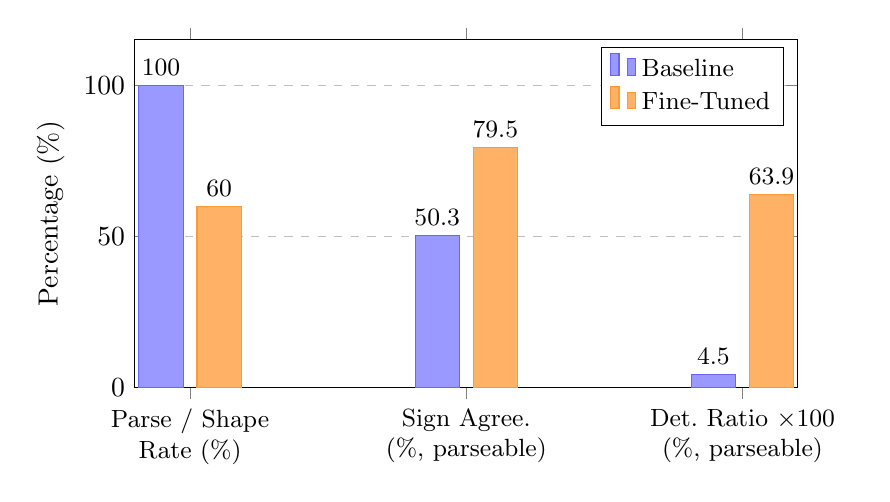
\begin{tikzpicture}
\begin{axis}[
    width=10cm,
    height=6cm,
    ylabel={Percentage (\%)},
    ybar=5pt,
    bar width=16pt,
    ymin=0,
    ymax=115,
    xtick=data,
    xticklabels={
        {Parse / Shape\\Rate (\%)},
        {Sign Agree.\\(\%, parseable)},
        {Det.\ Ratio $\times 100$\\(\%, parseable)}
    },
    x tick label style={font=\small, align=center, text width=2.8cm},
    legend style={at={(0.98,0.98)}, anchor=north east, font=\small},
    legend cell align={left},
    ymajorgrids=true,
    grid style=dashed,
    nodes near coords,
    nodes near coords align={vertical},
    every node near coord/.append style={font=\small},
]
\addplot[fill=blue!40, draw=blue!60] coordinates {
    (1, 100.0)
    (2, 50.3)
    (3, 4.5)
};
\addplot[fill=orange!60, draw=orange!80] coordinates {
    (1, 60.0)
    (2, 79.5)
    (3, 63.9)
};
\legend{Baseline, Fine-Tuned}
\end{axis}
\end{tikzpicture}

\vspace{0.8cm}

% --- Failure mode bar chart: fine-tuned model ---
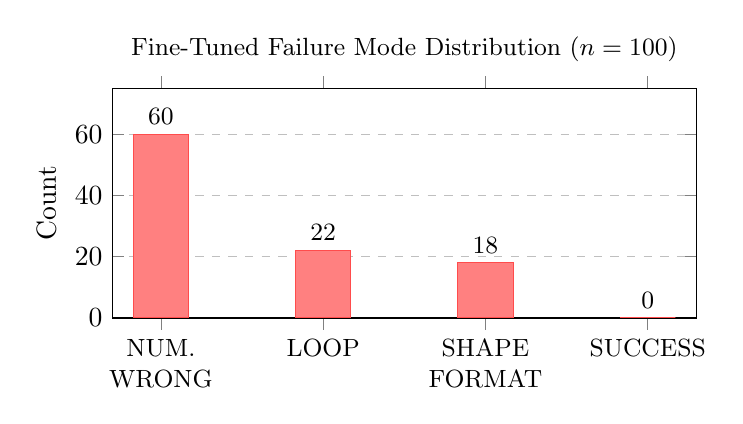
\begin{tikzpicture}
\begin{axis}[
    width=9cm,
    height=4.5cm,
    title={Fine-Tuned Failure Mode Distribution ($n = 100$)},
    title style={font=\small},
    ylabel={Count},
    ybar,
    bar width=20pt,
    ymin=0,
    ymax=75,
    xtick=data,
    xticklabels={
        {NUM.\\WRONG},
        {LOOP},
        {SHAPE\\FORMAT},
        {SUCCESS}
    },
    x tick label style={font=\small, align=center},
    ymajorgrids=true,
    grid style=dashed,
    nodes near coords,
    nodes near coords align={vertical},
    every node near coord/.append style={font=\small},
]
\addplot[fill=red!50, draw=red!70] coordinates {
    (1, 60)
    (2, 22)
    (3, 18)
    (4, 0)
};
\end{axis}
\end{tikzpicture}

\caption{
\textbf{Top}: Three normalized metrics (all higher = better) comparing baseline and fine-tuned model. Parse/shape rate measures generation reliability; sign agreement and determinant ratio ($\times 100$ for scale) measure inverse-like coarse structure among parseable outputs. Fine-tuning improves both structural metrics---sign agreement rises from 50.3\% to 79.5\%, determinant ratio from 4.5\% to 63.9\%---but reduces parse reliability by 40 percentage points. Additional diagnostics (residuals, relative Frobenius error, spectral error, copy distances) are in Table~\ref{tab:results}.
\textbf{Bottom}: Failure mode distribution for the fine-tuned model ($n = 100$ test examples). 60 outputs are parseable but numerically wrong; 22 loop until the token budget is exhausted; 18 produce malformed shapes; 0 achieve a successful inversion.}
\label{fig:results}
\end{figure}


\end{document}
